\documentclass[a4paper, 12pt]{report}

%%%%%%%%%%%%
% Packages %
%%%%%%%%%%%%

\usepackage[english]{babel}
\usepackage[noheader]{packages/sleek}
\usepackage{packages/sleek-title}
\usepackage{packages/sleek-theorems}
\usepackage{packages/sleek-listings}
\usepackage{longtable}

%%%%%%%%%%%%%%
% Title-page %
%%%%%%%%%%%%%%

\logo{figures/MicroGUI_logo.png}%figures/CLS_logo.png}
\institute{Canadian Light Source}
\faculty{FAR-IR Beamline}
%\department{Department of Anything but Psychology}
\title{The MicroGUI Project, V.0.2}
\subtitle{The horizontal microscope's user interface \& system integration program.}
\author{\textit{Author}\\Jai \textsc{Willems}}
\supervisor{\textit{Supervisor}\\Brant \textsc{Billinghurst}}
\date{\today}

%%%%%%%%%%%%%%%%
% Bibliography %
%%%%%%%%%%%%%%%%

\addbibresource{./resources/bib/references.bib}

%%%%%%%%%%
% Others %
%%%%%%%%%%

\lstdefinestyle{latex}{
    language=TeX,
    style=default,
    %%%%%
    commentstyle=\ForestGreen,
    keywordstyle=\TrueBlue,
    stringstyle=\VeronicaPurple,
    emphstyle=\TrueBlue,
    %%%%%
    emph={LaTeX, usepackage, textit, textbf, textsc}
}

\FrameTBStyle{latex}

\def\tbs{\textbackslash}

%%%%%%%%%%%%
% Document %
%%%%%%%%%%%%

\begin{document}
    \maketitle
    \romantableofcontents
    
    
    % ----------------------------------------------------------------------
    % Introduction
    % ----------------------------------------------------------------------


    \chapter{Introduction}
    % State the purpose of the document {Inform on the programs installation, function, and use.}
    % Background {motivation, intro line}
    % Expose the unknown (what unknown will be filled from the document).
    % Set up the rest {what will the remaining document express?}
    
    The MicroGUI project is a software development program for the horizontal infrared microscope of the Canadian Light Source's FAR-IR Beamline. This document is designed to present an overview of the program necessary for maintenance and consumer use.
    
    The original horizontal microscope control system consisted of three separate software components: the EDM GUI, Point Grey FlyCapture software, and the Thorlabs Kinesis software. From the different operating system requirements, the microscope's control became difficult and awkward. Thus, the prime motivator for the MicroGUI program, was the integration into a sole control software allowing for an improved and more professional user experience.
    
    In the remaining sections of this document, the program will be discussed from a user perspective, the setup/installation will be laid out, and the program's technical structure and code files will be broken down.
    
    
    % ----------------------------------------------------------------------
    % User Guide
    % ----------------------------------------------------------------------
    
    
    \chapter{User Guide}
    This section details the features of the MicroGUI interface along with their use.
    
    \begin{figure}[h]
        \centering
        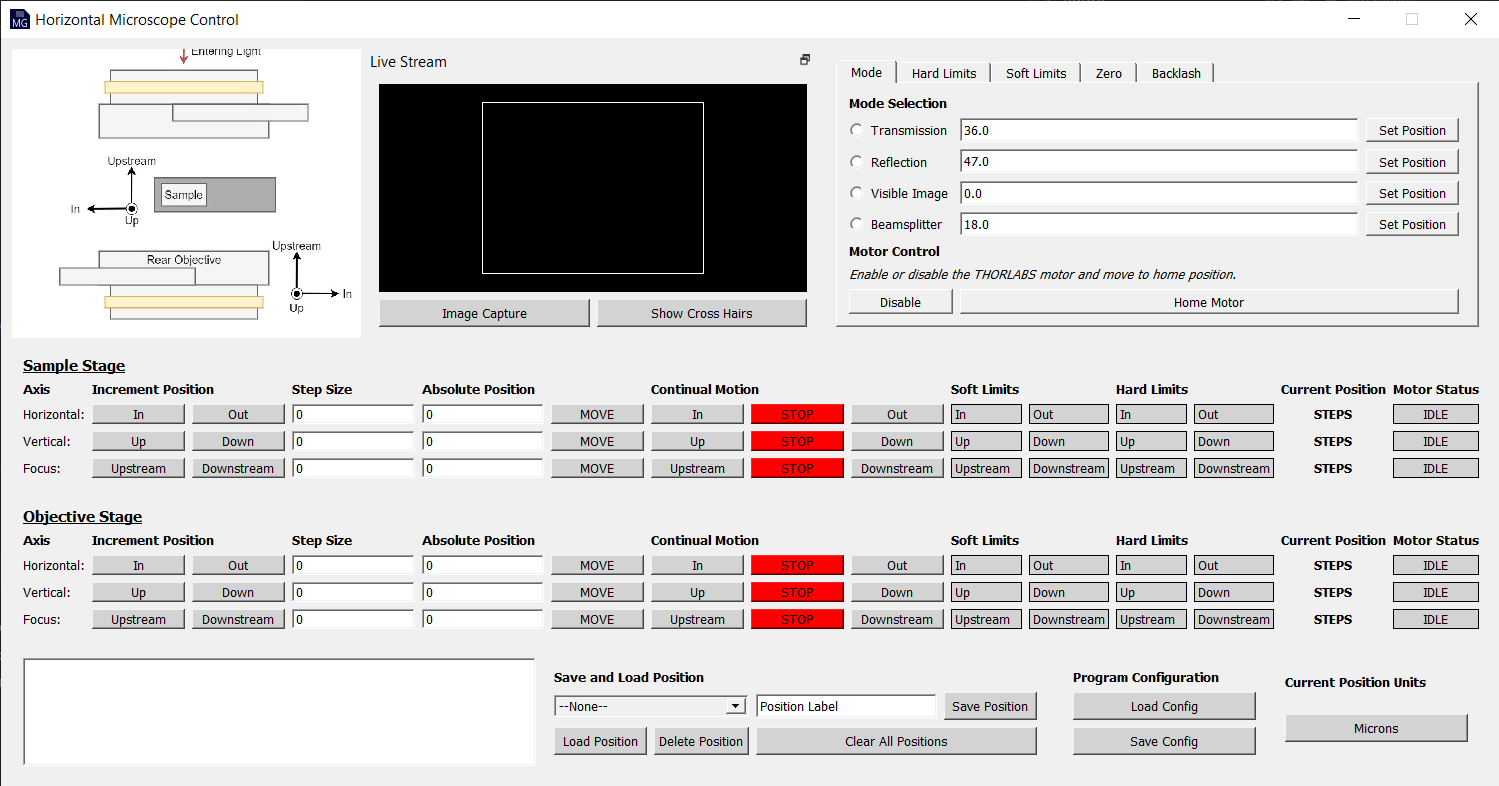
\includegraphics[width=0.9\textwidth]{figures/main_window.png}
        \caption{MicroGUI application.}
        \label{fig:1}
    \end{figure}
    
    
    \section{Diagram Window}
    \begin{figure}[h]
        \centering
        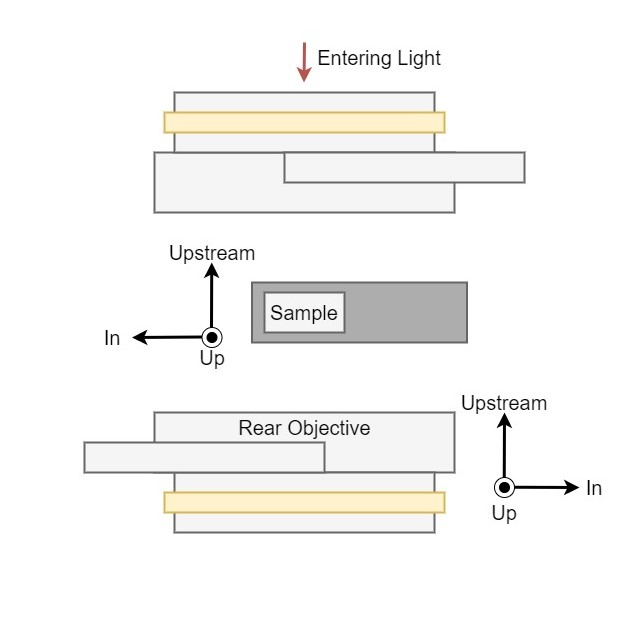
\includegraphics[width=0.5\textwidth]{figures/diagram.jpg}
        \caption{MicroGUI movement diagram.}
        \label{fig:2}
    \end{figure}
    
    The diagram window displays the image in figure \ref{fig:2} which defines the coordinate system of the microscope's controls. It defines the horizontal, vertical, and focus axes for the sample and objective stages. It also defines which directions are in and out, upstream and downstream, and up and down, respectively.
    
    \section{Live Feed Window}
    \begin{figure}[!tbph]
      \centering
      \begin{minipage}[b]{0.49\textwidth}
        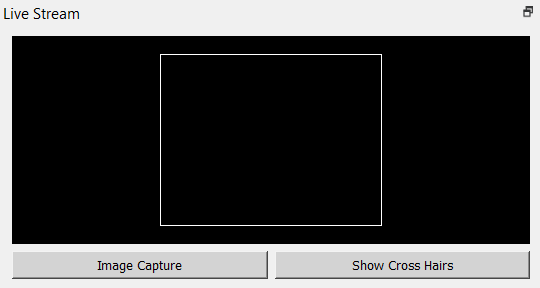
\includegraphics[width=\textwidth]{figures/camera_no_cross_hairs.png}
        \caption{Blank live feed, no cross hairs.}
        \label{fig:3}
      \end{minipage}
      \hfill
      \begin{minipage}[b]{0.49\textwidth}
        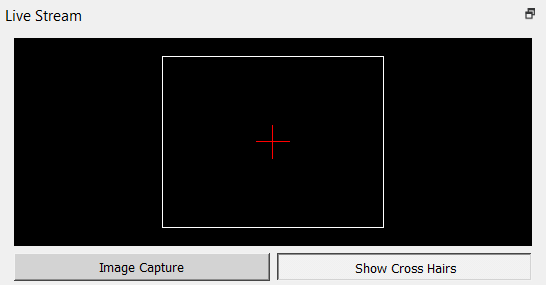
\includegraphics[width=\textwidth]{figures/camera_cross_hairs.png}
        \caption{Blank live feed, cross hairs.}
        \label{fig:4}
      \end{minipage}
    \end{figure}

    The live feed window provides a direct user interface with the FLIR/Point Grey Blackfly USB3 Camera (as seen in figures \ref{fig:3} and \ref{fig:4}). The display has four main components:
    
    \begin{enumerate}
        \item The display includes a viewing window (demonstrated by the white border in the figures) that surrounds the camera display to allow users to change the size and position of the live feed. The feed size can be changed by using a mouse scroll wheel while hovering over the feed. The feed can also be panned by clicking and dragging the feed.
        \item Optional crosshairs allow users to track motion and localize on certain objects. The crosshairs can be toggled on or off using the \textit{Show Cross Hairs} toggle button.
        \item An image capture button which, when pressed, will open up a secondary window to allow users to choose the saving directory and filename. Note that the crosshairs will be added to the image if present on the feed display.
        \item An enlarged view functionality is available by clicking the \textit{Restore Down} button in the live feeds upper right corner or by double clicking the feed window header. This will detach the feed from the main user interface and allow users to enlarge the window by clicking and dragging the window bounds. To return the live feed to the GUI, double click on the live feed's window header.
    \end{enumerate}
    
    
    \section{Tab Window}
    The tab window contains four tabs containing less frequently interfaced information yet still essential to access.
    
    \subsection{Mode Tab}
    \begin{figure}[h]
        \centering
        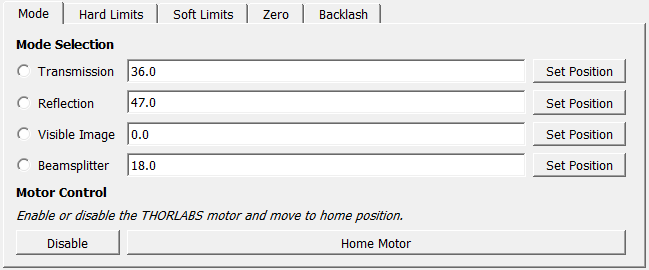
\includegraphics{figures/thorlabs_mode_tab.png}
        \caption{Mode tab.}
        \label{fig:5}
    \end{figure}
    
    The mode tab, as seen in figure \ref{fig:5} provides the necessary controls to change the microscope mode and calibrate mode positions.
    
    There are four mode selection buttons to select between the reflection, transmission, visible image, and beamsplitter modes. The positions associated with each mode can be altered using the adjacent line edits. To change a mode position, change the modes adjacent line edit (in mm) before selecting the \textit{Set Position} button to save the input position value to the internal database.\footnote{The internal data base is separate from the configuration file handling. To ensure the changes will persist after closing the program, the configuration file will need to be saved.} If the mode position being changed is selected, the motor will automatically adjust to the newly set position.
    
    The bottom of the mode tab has additional motor controls, which will be of no concern to users. These buttons allow one to enable or disable the Thorlabs motor as well as move the motor to its \textit{home} position. These controls are present for the beamline staff for when the Thorlabs motor is inoperative. Note that the motor must be enabled to change modes or home successfully or else an error will be returned.
    
    
    \subsection{Hard Limits Tab}
    \begin{figure}[h]
        \centering
        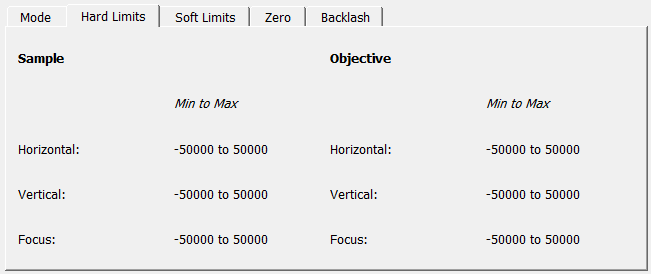
\includegraphics{figures/hard_limits_tab.png}
        \caption{Hard limits tab.}
        \label{fig:6}
    \end{figure}
    
    The hard limits tab, as seen in figure \ref{fig:6} details the range of motion for each of the sample/objective motors. These limits are defined by the physical limitations to a motors motion and are displayed primarily for the scale of motion and user insight. Note that the hard limit values are given in steps.
    
    
    \subsection{Soft Limits Tab}
    \begin{figure}[h]
        \centering
        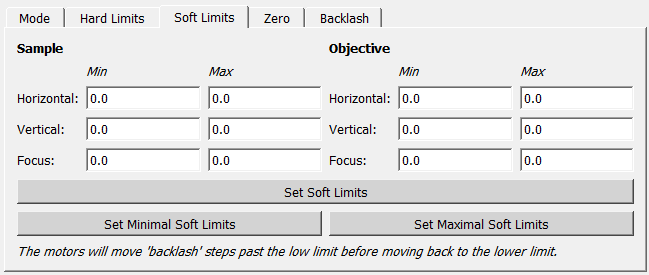
\includegraphics{figures/soft_limits_tab.png}
        \caption{Soft limits tab.}
        \label{fig:7}
    \end{figure}

    The soft limits tab, as seen in figure \ref{fig:7} allows one (beamline staff) to set soft limits on the program to prevent possible hardware collisions. Such limits can be set in three ways:
    
    \begin{enumerate}
        \item The \textit{Set Soft Limits} button will set the soft limits to the values inputted into the 12 text boxes. If an inputted soft limit value is more extreme than its corresponding hard limit value, then the soft limit will be set to the hard limit. All motors that fall outside of the new limits will automatically be moved to the closest limit and the soft limitds illuminated. Additionally, the minimum soft limit must be less than the maximum soft limit or an error will be returned.
        \item The \textit{Set Minimum Soft Limits} button will set all soft limits to zero. All motors that fall outside of the new limits will automatically be moved to the zero position and soft limit indicators will be updated.
        \item The \textit{Set Maximum Soft Limits} button will set all soft limits to the corresponding hard limit values (indicated on the hard limits tab) to effectively remove any soft limit constraints. This method is not recommended as the soft limits provide a safety margin against hardware collisions. Only use this functionality if on-site and in the visual range of the microscope setup.
    \end{enumerate}
    
    Note that soft limits are interfaced in units of steps.

    
    \subsection{Zero Tab}
    \begin{figure}[h]
        \centering
        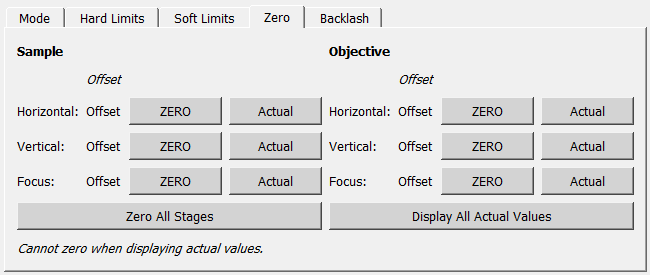
\includegraphics{figures/zero_tab.png}
        \caption{Zero tab.}
        \label{fig:8}
    \end{figure}

    The zero tab seen in figure \ref{fig:8} allows users to manipulate the data display to provide convenient positions relative to a user-defined datum. This tab contains several controls:
    
    \begin{enumerate}
        \item The \textit{ZERO} button functionality allows users to zero the position of a stage motor to create a new datum. Zeroing will change the soft limits, hard limits, stage offset, and current position to reflect the new zeroed position. Similarly, the \textit{Zero All Stages} button zero's all stage motors.
        \item The \textit{Actual} button functionality changes a zeroed display value to show actual values (positions with reference to an internally defined datum). Thus, the offset will be removed and related position displays will be updated to reflect the re-established datum. Similarly, the \textit{Display All Actual Values} button reverts the zeroing of all stage motors.
    \end{enumerate}
    
    \subsection{Backlash Tab}
    \begin{figure}[h]
        \centering
        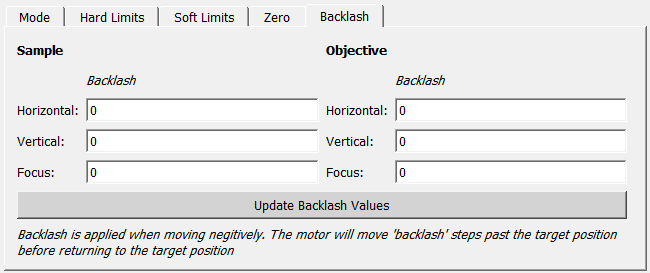
\includegraphics{figures/backlash_tab.png}
        \caption{Backlash tab.}
        \label{fig:11}
    \end{figure}

    The backlash tab seen in figure \ref{fig:11} allows users to manipulate the motors' backlash parameters for best performance.
    
    Backlash line edits and the \textit{Set Backlash Values} button allow users to define and save new backlash values for each stage motor. Inputted values represent steps and must be positive integer values. It is recommended that users do not change default values that have been proven through testing to be optimal.
    
    
    \section{Sample \& Objective Windows}
    \begin{figure}[h]
        \centering
        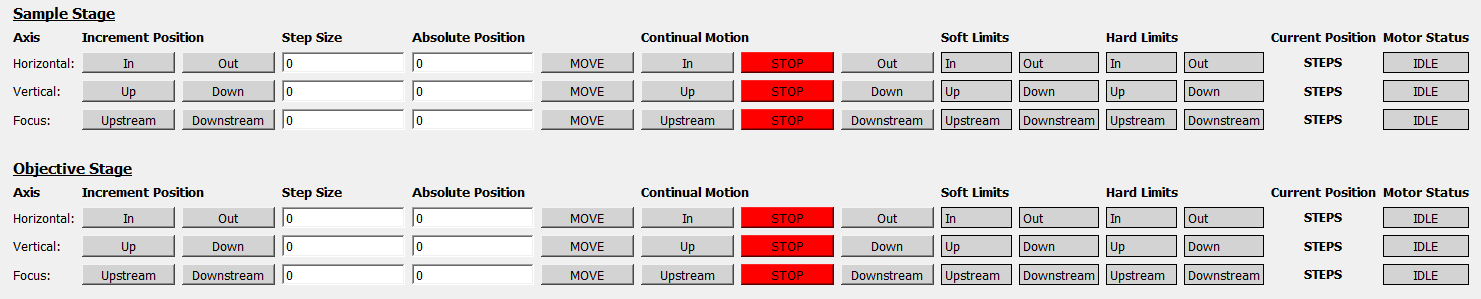
\includegraphics[width=\textwidth]{figures/sample_objective_window.png}
        \caption{Sample and objective control windows.}
        \label{fig:9}
    \end{figure}

    The sample and objective windows have similar controls and nearly identical functionality. As a result, the information in this section can be generalized to both displays. Note that positive and negative will be used to generalize the motor direction labels (e.g.in, out, upstream, etc.) for the sake of simplicity.
    
    The displays can be broken into four main sections: three-movement forms (incremental, absolute, and continuous positioning) and one for motor status.
    
    \begin{enumerate}
        \item The sample and objective stage motors can be moved with precision using the increment-position controls. These controls include incremental positive and negative buttons in addition to a step-size input. The step size indicates the size of each increment in steps, and the incremental position buttons indicate the direction to move the stage. These methods are ideal for precise motor control.
        \item The sample and objective stage motors can also be moved to an absolute position using the absolute position controls. An absolute position can be inserted into the \textit{Absolute Position} line edit, and the \textit{MOVE} button can be pressed to start motor motion. This control sequence is recommended when using predefined positions. Note that a newly input value is not internally known to the program until the move button is pressed.
        \item The final type of motion is continuous. The continuous motion controls include the continuous positive, continuous negative, and \textit{STOP} buttons. Pressing the continuous positive or continuous negative push buttons will begin the stage motor's motion in the defined direction. Such motion will continue until a soft/hard limit is reached, or the \textit{STOP} button is pressed. This form of control is ideal when coarse movements are desirable.
        \item The sample and objective stages also encapsulate several status indicators, including soft and hard limits, current position feedback, and motor status labels.
        \begin{enumerate}
            \item The soft or hard limit labels will illuminate green if their respective soft or hard limits are met. When a specific limit is not met, it will default to light grey.
            \item The \textit{Current Position} feedback display updates continuously to give the most up-to-date position of the motor. The current position can be toggled between units of steps and microns as will be discussed in section \ref{miscellaneous_window}.
            \item The motor status label indicates the current state of the motor. The possible states include idle, powering, powered, releasing, active, applying, and unpowering.
        \end{enumerate}
    \end{enumerate}
    
    \section{Miscellaneous Window}\label{miscellaneous_window}
    \begin{figure}[h]
        \centering
        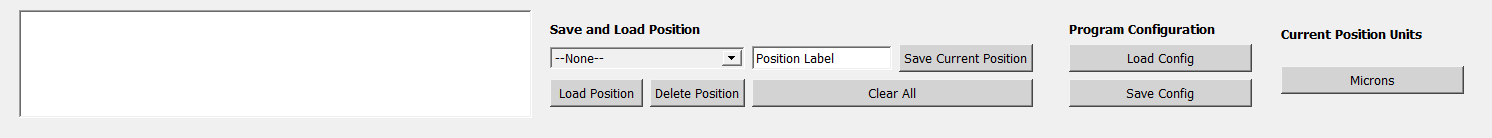
\includegraphics[width=\textwidth]{figures/miscelaneous_tab.png}
        \caption{Miscellaneous window.}
        \label{fig:10}
    \end{figure}
    
    The bottom of the GUI represents the miscellaneous tab with categorized functionality consisting of four main sections:
    \begin{enumerate}
        \item The \textit{Program Status Console} is the largest widget on the miscellaneous window, which prints out statements throughout the program's operation. These messages provide confirmation of user actions and provide warnings and errors should they arise. For this program, \textit{warnings} are defined as changes the GUI has made to a user action to adhere to internal rules that do not inhibit the program but may change the expected outcome. Warnings will be displayed in yellow text. An \textit{error} is defined as inhibited GUI functionality due to command incompatibility with the software/hardware. Errors will be displayed in red text. Some error messages will give ideas about potential corrective actions to take.
        \item The \textit{Save and Load Position} section allows the user to store and restore positions of interest. There are four main parts of the \textit{Save and Load Position} section.
        \begin{enumerate}
            \item A user can save the current sample and objective positions by adding in a position label and pressing the \textit{Save Current Position} button. Note that position labels must be unique and will throw an error if a duplicate label is inserted.
            \item A user can load a saved position by selecting the desired position from the position drop down menu and pressing the \textit{Load Position} button.
            \item A user can delete a saved position by selecting the desired position from the position drop down menu and pressing the \textit{Delete Position} button.
            \item Lastly, a user can clear all saved positions by pressing the \textit{Clear All} button.
        \end{enumerate}
        \item The miscellaneous tab also contains \textit{Program Configuration} controls. The \textit{Load Config} button allows a user to upload a previous program configuration, whereas the \textit{Save Config} button allows a user to save the current configuration.
        \item Lastly, the \textit{Microns} button toggles the sample and objective \textit{Current Position} displays between units of steps and micrometres.
    \end{enumerate}
    
    
    % ----------------------------------------------------------------------
    % Program Environment and Installation
    % ----------------------------------------------------------------------
    
    
    \chapter{Program Environment \& Installation}
    
    The MicroGUI program has a series of dependencies that require installation and configuration before the program can be successfully executed. This chapter will detail the steps to fully set up the necessary program dependencies and initialize the program launcher and the program itself.
    
    \section{Dependencies}
    The program requires various dependencies, including a specific Python installation, various package downloads, THORLABS motor stage dependencies, and the FLIR/BlackFly camera dependencies. The following subsections will outline such configuration.

    \subsection{Python Environment}\label{PYTHONconfig}
    The coding environment for the MicroGUI program is Python and will need to be installed. For the coding environment to be compatible with the later installed dependencies, a version of Python 3.8.10 is recommended and can be downloaded \href{https://www.python.org/downloads/release/python-3810/}{here}.
    
    Once the python environment is set up, we need to install the MicroGUI files. To do this, open up git bash and navigate the directory tree using the \verb|cd| command to the location where the program will reside. Then, clone the MicroGUI repository using the following command:
    
    \begin{verbatim}
        git clone https://github.com/JaiWillems/MicroGUI.git
    \end{verbatim}
    
    If git bash is not installed on the current computer, then download the repositories ZIP folder\footnote{Ensure you are cloning from the master branch as this will be the most current stable version.} containing all project files \href{https://github.com/JaiWillems/MicroGUI}{here}. Unzip the downloaded folder to the path of interest.
    
    Note that this GitHub repository will no longer be updated as of August 27th 2021 and the CLS Enterprise GitHub should be used to source the most up to date files.
    
    Next, we need to install the Python dependencies required by the MicroGUI program. To download the dependencies, open the windows command prompt and navigate to the MicroGUI directory where the \verb|requirements.txt| file is located. Run the following command:
    
    \begin{verbatim}
        pip install -r requirements.txt
    \end{verbatim}
    
    This command will install the appropriate versions of the package dependencies to the current Python environment necessary for the seamless operation of the MicroGUI software.
    
    This concludes the Python environment setup.
    
    
    \subsection{Thorlabs Dependency Configuration}
    The horizontal microscope setup contains a Thorlabs motor used for mode selection. This section details the steps to configure the Thorlabs motor environment.
    
    To begin, download and install the Thorlabs APT software found \href{https://www.thorlabs.com/software_pages/ViewSoftwarePage.cfm?Code=Motion_Control&viewtab=1}{here} that corresponds to the system architecture and Python version (Python 3.8.10). This software is necessary for allowing the python modules to interface with the motors firmware.
    
    Lastly, a small configuration of the \textit{thorlabs\_apt} Python library folder (downloaded in section \ref{PYTHONconfig}) must occur to ensure proper dependencies are accessible. To accomplish this configuration, navigate the file system to find the \textit{APT.dll} file from the Thorlabs APT software. The default installation will result in the \textit{APT.dll} file being found in the following path, \verb|C:/Program Files/Thorlabs/APT/APT Server|. Paste this file in the \textit{thorlabs\_apt} directory located within the Python directory (\verb|...\Python\Python38\Lib\site-packages|).
    
    This concludes the Thorlabs motor environment setup.


    \subsection{FLIR Dependency Configuration}\label{FLIRconfig}
    To interface with the BlackFly USB3 camera, we will need to download and install two pieces of software: the Spinnaker SDK and the latest Python Spinnaker, both are found \href{https://flir.app.boxcn.net/v/SpinnakerSDK}{here}. 
    
    
    \subsubsection{Spinnaker SDK}
    Navigate the FLIR downloads directory into the appropriate operating system and download the \verb|Latest Spinnaker Full SDK| file. Once downloaded, run the executable's installation corresponding to your system architecture (e.g. \verb|SpinnakerSDK_FULL_2.4.0.144_x64.exe|.
    
    
    \subsubsection{Python Spinnaker}
    Navigate the FLIR downloads directory to the appropriate operating system, open the \verb|Latest Python Spinnaker| folder, then download and unzip the latest Python Spinnaker (PySpin) folder that matches the installed Python version. For Python 3.8 on a Windows 64 machine, the appropriate folder is \verb|spinnaker_python-2.4.0.143-cp38-cp38-win_amd64.zip|).
    
    The PySpin library can then be installed from the Python WHL file located in the just downloaded PySpin directory. To accomplish the download, use the following commands in a terminal to navigate to the PySpin directory and install the WHL file:
    
    \begin{verbatim}
        cd <PySpin_whl_unzip_destination>
        pip install --user <PySpin_whl_file>
    \end{verbatim}
    
    This concludes the FLIR camera environment setup.
    
    
    \section{Producing the MicroGUI Launcher}\label{launcher_exe}
    The MicroGUI is initialized using an executable file dubbed the MicroGUI Launcher. This section will detail the steps to create a new launcher executable file if the MicroGUI files' directory tree is altered.
    
    The \verb|run.py| file is simple and only contains three lines of code:
    
    \begin{verbatim}
        import os
        os.chdir("C:/Users/Public/Documents/MicroGUI/microgui/source"
        os.system("python main.py")
    \end{verbatim}
    
    For the run file to be properly configured, the path passed into the \verb|os.chdir()| function must be the path to the MicroGUI's \verb|main.py| file. Once the run file has the appropriate path, navigate the command prompt to MicroGUI's source folder using the \verb|cd| command and use the following command (assuming the \verb|PyInstaller| package was downloaded in section \ref{PYTHONconfig}):
    
    \begin{verbatim}
        pyinstaller --noconfirm --onedir --windowed --icon <icon path> --name
        "MicroGUI Launcher" <output path>
    \end{verbatim}
    
    This will produce the output executable and accompanying files to the \verb|<output path>|. A shortcut can then be made to copy the executable to the desktop.


    \section{Program Operation}
    At this point, all necessary dependencies are installed, and we are ready to run the program.
    
    Begin by ensuring \textbf{all Thorlabs and FLIR/BlackFly software are closed} as their operations have been found to prevent access to external hardware from the MicroGUI software. Additionally, check that any other motor control programs for the horizontal microscope are closed, their presence can prevent the MicroGUI program from writing to process variables. Then, check that the camera and Thorlabs motors are connected to the computer (they will need to be connected before program initiation).
    
    There are two main methods of program initialization: using the launcher or the command line. If there exists a current MicroGUI Launcher, double-click the launcher to activate the program. To initialize the program from the command line, navigate the terminal to the project repository (downloaded in section \ref{PYTHONconfig}). Type the command \verb|python main.py| to initialize the program. In both cases, the program will take a moment to start up. Once the GUI has appeared, you will be ready to use the software to interface with the horizontal microscope.
    
    \section{Uploading a New Releases to the CLS Computer}
    
    The interaction between the MicroGUI launcher and source code files is a weird yet simple one. The launcher was created to produce a series of terminal commands to launch the \verb|main.py| project file stored in \verb|C:/Users/Public/Documents/MicroGUI/microgui/source| path. There are two ways to deploy a new version of the program.
    
    \begin{enumerate}
        \item The first is to download the program from GitHub and create a new executable with an updated path to the new versions \verb|main.py| file.
        \item The second option is to directly replace the MicroGUI program files with the new release. Since the executable runs the \verb|main.py| file from a specific path, no new executable will be necessary so long as the \verb|main.py| file is located in the \verb|C:/Users/Public/Documents/MicroGUI/microgui/source| directory.
    \end{enumerate}
    
    
    % ----------------------------------------------------------------------
    % MicroGUI Code
    % ----------------------------------------------------------------------
    
    
    \chapter{MicroGUI Code}
    \section{File and Class Structure}
    The program is separated into eight source code files that combine to give the user the functionality they desire.
    \begin{itemize}
        \item The \verb|main.py| file initiates and closes the program by invoking all necessary files to work in combination to create the user interface and underlying functionality.
        \item The \verb|gui.py| file contains the \verb|GUI|, \verb|CameraWindow|, and \verb|MyTableWidget| class' which are responsible for creating the user interface. The \verb|GUI| class is the main object for the user display. The \verb|CameraWindow| class is the object governing the detachable camera window. The \verb|MyTableWidget| class is used to create the tab window on the main user interface display.
        \item The \verb|controller.py| file contains the \verb|Controller| class which adds the functionality to the user interface by connecting the interactive widgets created by the \verb|GUI| class to control sequences to invoke change in the microscope or display.
        \item The \verb|configuration.py| file provides the functions necessary for loading and saving the program configuration files and the saved-positions configuration file.
        \item The \verb|config.json| file stores the default macro variables that are uploaded on program start up. Note that other configurations can be loaded after the program has begun.
        \item The \verb|saved_positions.json| file stores the programs saved positions. 
        \item The \verb|thorlabs_motor_control.py| file provides the functions necessary to control the Thorlabs motor.
        \item The \verb|flir_camera_control.py| file provides the function to acquire images from the FLIR/BlackFly camera.
        \item The \verb|run.py| file can be converted into an executable to launch the MicroGUI program through a series of terminal commands. Refer to section \ref{launcher_exe} for details on the generation of the executable file.
    \end{itemize}
    
    
    \section{Imported Modules}
    
    This section details the various module imports used throughout the program. For each import, a brief description of its use and a reference to documentation will be given.
    
    For simplicity, only non-trivial and uncommon packages will be documented.
    
    \subsection{PyQt5}
    
    The PyQt5 package is a high-level API package used for the entire user interface. The documentation for the Python-based version is given \href{https://doc.bccnsoft.com/docs/PyQt5/}{here}.
    
    \subsection{PyQtGraph}
    
    The PyQtGraph package is a Python graphics and user interface package derived from PyQt5. It is used solely for the camera live feed in the MicroGUI program. Its documentation can be found \href{https://pyqtgraph.readthedocs.io/en/latest/}{here}.
    
    \subsection{PyEpics}
    
    The PyEpics package allows one to interface with an EPICS control system to enact changes to process variables. The package was used for all EPICS interactions. Its documentation can be found \href{https://pyepics.github.io/pyepics/overview.html}{here}.
    
    \subsection{thorlabs\_apt}
    
    The thorlabs\_apt package allows for interfacing with the Thorlabs motors. It is used to control the microscopes Thorlabs motor for mode control. Its documentation can be found \href{https://github.com/qpit/thorlabs_apt}{here}.

    \subsection{simple-pyspin}
    
    The simple-pyspin package is used as a simplified approach to interface with the programs BlackFly Camera instead the original Python Spinnaker. The documentation can be found \href{https://klecknerlab.github.io/simple_pyspin/}{here}.

\end{document}
